% !TEX root = ../slides.tex
%%%%%%%%%%%%%%%%%%%%%%%%%%%%%%%%%%%%%%%%%%%%%%%%%%%%%%%%%%%%%%%%%%%%%%%%%%%%%%%%
% Session 1: Weak formulation
%%%%%%%%%%%%%%%%%%%%%%%%%%%%%%%%%%%%%%%%%%%%%%%%%%%%%%%%%%%%%%%%%%%%%%%%%%%%%%%%

\session{session01}{Galerkin's method}{Weak formulation}
{Sections 1.1.1--1.1.5}
{\notebook{lectures/galerkin}{FEMlinear1dLaplaceDirichlet.ipynb}}
{1.1--1.6}

\begin{frame}{Plan for today}
    \begin{enumerate}
        \item From the PDE to a variational (weak) problem.
        \item Existence and uniqueness: the Lax--Milgram theorem.
        \item From bilinear forms to operators.
        \item Galerkin discretisation: replace $V$ by a finite-dimensional $V_h$.
        \item Linear algebra: the stiffness matrix.
    \end{enumerate}
    \bigskip
    \takeaway{Idea of Galerkin's method: see the PDE as an equation in an infinite-dimensional space, and move it to a finite-dimensional subspace, where it can be solved.}
    \medskip
    {\small (Finite differences instead see the PDE as relations between derivatives, and replace them by difference quotients.)}
\end{frame}

\begin{frame}{Model problem: Laplace's equation}
    \[
        -\Delta u = f \quad \text{in } \Omega.
    \]
    Multiply by a test function $v$ and integrate by parts ($u \in C^2(\overline\Omega)$, $v \in C^1(\overline \Omega)$):
    \[
        \int_\Omega (-\Delta u)\, v = \int_\Omega \nabla u \cdot \nabla v - \int_{\partial \Omega} v\, \nabla u \cdot n.
    \]
    \begin{itemize}
        \item The boundary term vanishes if $v = 0$ on $\partial\Omega$ (Dirichlet) or if $\nabla u \cdot n = 0$ on $\partial\Omega$ (Neumann).
        \item We are left with the bilinear form
              \[
                  a_L(u,v) \defeq \int_\Omega \nabla u \cdot \nabla v .
              \]
        \item Only \alert{first derivatives} of $u$ are needed: natural space $H^1(\Omega)$.
    \end{itemize}
\end{frame}

\begin{frame}{Two examples in $d = 1$}
    \small
    \begin{example}[Laplace with Dirichlet conditions]
        \[
            -u'' = f \text{ in } (0,1), \qquad u(0) = u(1) = 0.
        \]
        Weak formulation: find $u \in H^1_0(0,1)$ such that
        \[
            \int_0^1 u' v' = \int_0^1 f v \qquad \forall v \in H^1_0(0,1).
        \]
    \end{example}
    \begin{example}[Helmholtz with Neumann conditions]
        \[
            -u'' + u = f \text{ in } (0,1), \qquad u'(0) = u'(1) = 0.
        \]
        Weak formulation: find $u \in H^1(0,1)$ such that
        \[
            \int_0^1 u' v' + \int_0^1 u v = \int_0^1 f v \qquad \forall v \in H^1(0,1).
        \]
    \end{example}
    {\small Dirichlet conditions go into the space $V$; Neumann conditions are hidden in the formulation.}
\end{frame}

\begin{frame}{The abstract problem}
    Let $V$ be a Hilbert space, $a : V \times V \to \R$ bilinear and $\ell : V \to \R$ linear.
    \[
        \tag{E}
        \text{Find } u \in V \text{ such that } a(u,v) = \ell(v) \qquad \forall v \in V.
    \]
    \begin{itemize}
        \item Laplace--Dirichlet: $V = H^1_0(0,1)$, $a(u,v) = \int_0^1 u'v'$, $\ell(v) = \int_0^1 fv$.
        \item Helmholtz--Neumann: $V = H^1(0,1)$, $a(u,v) = \int_0^1 (u'v' + uv)$, $\ell(v) = \int_0^1 fv$.
    \end{itemize}
    \board{Exercise 1.1: if a weak solution is $C^2(\overline\Omega)$, then it is a classical solution (integrate by parts back and choose $v$ well).}
\end{frame}

\begin{frame}{Existence and uniqueness}
    \begin{theorem}[Lax--Milgram]
        Let $V$ be a Hilbert space, $a: V\times V \to \R$ bilinear and $\ell \in V^*$. Assume
        \begin{enumerate}
            \item continuity: $|a(u,v)| \le M \|u\|_V \|v\|_V$,
            \item coercivity: $a(u,u) \ge \alpha^* \|u\|_V^2$ with $\alpha^* > 0$.
        \end{enumerate}
        Then \textup{(E)} has a unique solution $u \in V$. Moreover $\|u\|_V \le \frac{1}{\alpha^*}\|\ell\|_{V^*}$.
    \end{theorem}
    \begin{proofsteps}[Idea of the proof (symmetric case)]
        If $a$ is also symmetric, $a(\cdot,\cdot)$ is a scalar product on $V$ with norm equivalent to $\|\cdot\|_V$.
        Then \textup{(E)} is exactly the Riesz representation theorem for $\ell$ in $(V, a)$.
        The general case uses Riesz and a fixed-point argument; see Brezis, Corollary 5.8.
    \end{proofsteps}
\end{frame}

\begin{frame}{Applying Lax--Milgram (Exercise 1.2)}
    \textbf{Continuity.} By the Cauchy--Schwarz inequality,
    \[
        \left|\int_0^1 u'v'\right| \le \|u'\|_{L^2}\|v'\|_{L^2} \le \|u\|_{H^1}\|v\|_{H^1}, \qquad
        \left|\int_0^1 f v\right| \le \|f\|_{L^2}\|v\|_{H^1}.
    \]
    \textbf{Coercivity.}
    \begin{itemize}
        \item Helmholtz: $a(u,u) = \|u'\|_{L^2}^2 + \|u\|_{L^2}^2 = \|u\|_{H^1}^2$, so $\alpha^* = 1$.
        \item Laplace--Dirichlet: we need Poincaré's inequality
              \[
                  \|v\|_{L^2(0,1)} \le \frac 1 \pi \|v'\|_{L^2(0,1)}, \qquad v \in H^1_0(0,1),
              \]
              so that $a(u,u) = \|u'\|^2_{L^2} \ge \left(1+\frac{1}{\pi^2}\right)^{-1} \|u\|_{H^1}^2$.
    \end{itemize}
    \board{Neumann problem for $-u'' = f$ (Exercise 1.3): there is no coercivity in $H^1$ (constants!). Work in $V = \{u \in H^1 : \int_0^1 u = 0\}$.}
\end{frame}

\begin{frame}{From bilinear forms to operators}
    Let $V \subset H$ be Hilbert spaces, with $V$ dense and continuously embedded in $H$ (e.g.\ $H^1_0 \subset L^2$).
    \begin{definition}[Operator associated to $a$]
        \[
            D_H(A) = \Big\{ u \in V : \sup_{v \in V\setminus\{0\}} \frac{|a(u,v)|}{\|v\|_H} < \infty \Big\}.
        \]
        For $u \in D_H(A)$, the Riesz theorem in $H$ gives $Au \in H$ such that
        \[
            \prodH{Au}{v} = a(u,v) \qquad \forall v \in V.
        \]
    \end{definition}
    \begin{example}[Dirichlet Laplacian in $(0,1)$]
        $V = H^1_0(0,1)$, $H = L^2(0,1)$, $a(u,v) = \int_0^1 u'v'$. Then $A = -\Delta_D$ and
        $D_{L^2}(-\Delta_D) = H^2(0,1) \cap H^1_0(0,1)$.
    \end{example}
\end{frame}

\begin{frame}{Weak formulation $=$ functional equation}
    \begin{lemma}
        Assume $V$ is dense in $H$ and $\ell(v) = \prodH{f}{v}$ with $f \in H$. Then $u \in V$ solves \textup{(E)} if and only if
        \[
            u \in D_H(A) \quad \text{and} \quad Au = f \text{ in } H.
        \]
    \end{lemma}
    \begin{proofsteps}
        \begin{enumerate}
            \item[$\Rightarrow$] $|a(u,v)| = |\prodH{f}{v}| \le \|f\|_H \|v\|_H$, so $u \in D_H(A)$.
            \item[] Then $\prodH{Au - f}{v} = 0$ for all $v \in V$.
            \item[] By density of $V$ in $H$, also for all $v \in H$. Hence $Au = f$.
            \item[$\Leftarrow$] $a(u,v) = \prodH{Au}{v} = \prodH{f}{v} = \ell(v)$.
        \end{enumerate}
    \end{proofsteps}
    \takeaway{We will use $A$ to measure regularity: e.g.\ $\|Au\|_H = \|u''\|_{L^2}$.}
\end{frame}

\begin{frame}{Galerkin discretisation}
    Take a \alert{finite-dimensional subspace} $V_h \subset V$ and solve
    \[
        \tag{E$_h$}
        \text{Find } u_h \in V_h \text{ such that } a(u_h,v_h) = \ell(v_h) \qquad \forall v_h \in V_h.
    \]
    \begin{itemize}
        \item $V_h$ is also a Hilbert space, and $a$ is still continuous and coercive on $V_h$.
        \item By Lax--Milgram, there exists a unique $u_h \in V_h$.
        \item $h$ is a discretisation parameter: we want $u_h \to u$ as $h \to 0$.
    \end{itemize}
    \bigskip
    \takeaway{Main questions of the course: good choices of $V_h$, and estimates of $\|u - u_h\|$ in different norms.}
\end{frame}

\begin{frame}{Example: piece-wise linear functions in $d=1$}
    \begin{columns}[T]
        \begin{column}{.58\textwidth}
            Mesh $0 = x_0 < x_1 < \cdots < x_N = 1$, $h_i = x_i - x_{i-1}$, $h = \max_i h_i$.
            \[
                \varphi_i(x) =
                \begin{cases}
                    \dfrac{x - x_{i-1}}{h_i}     & x \in (x_{i-1}, x_i],  \\[1ex]
                    \dfrac{x_{i+1} - x}{h_{i+1}} & x \in (x_i, x_{i+1}],   \\[1ex]
                    0                            & \text{otherwise.}
                \end{cases}
            \]
            (at $x_0$ and $x_N$ keep only the piece inside $[0,1]$).
        \end{column}
        \begin{column}{.38\textwidth}
            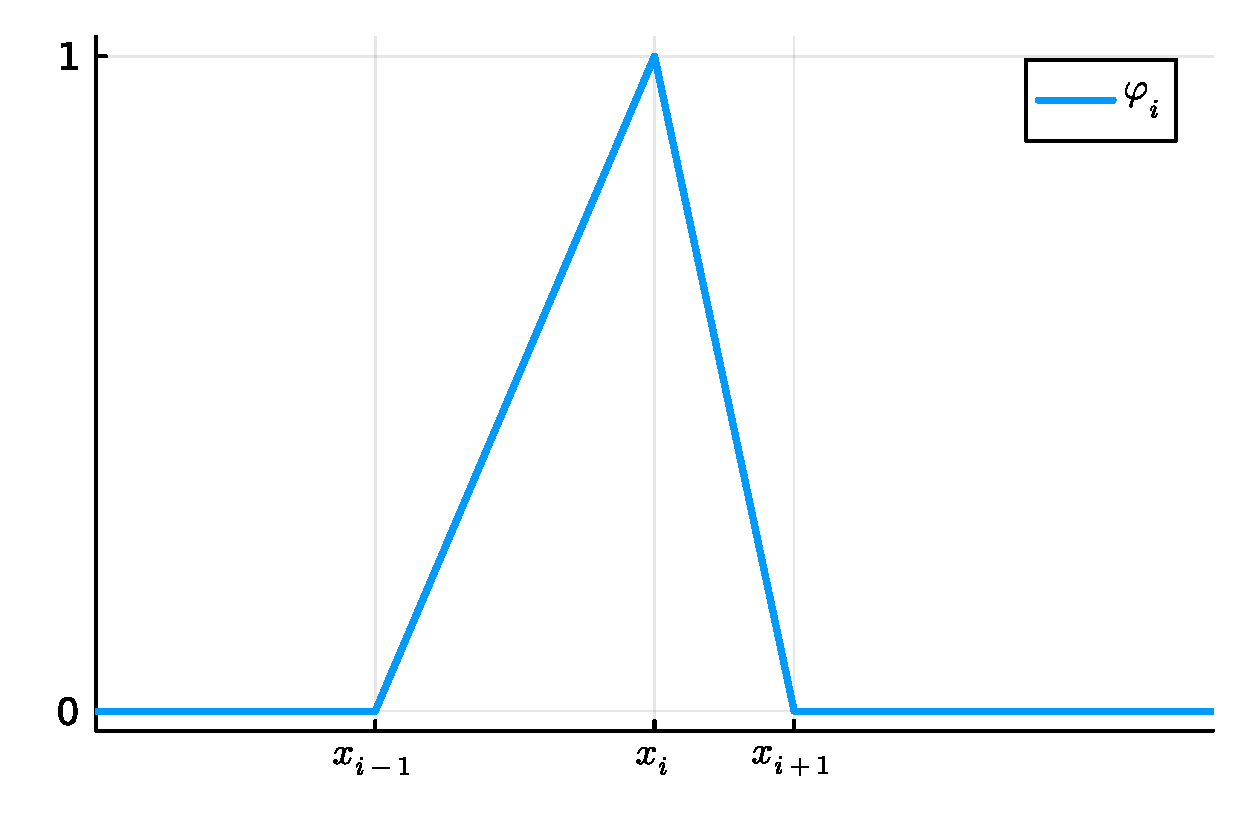
\includegraphics[width=\textwidth]{../../lectures/galerkin/figures/basis-function.pdf}
        \end{column}
    \end{columns}
    \medskip
    \begin{itemize}
        \item $V = H^1(0,1)$ (Neumann): $V_h = \spannedby\{\varphi_0, \dots, \varphi_N\}$.
        \item $V = H^1_0(0,1)$ (Dirichlet): $V_h = \spannedby\{\varphi_1, \dots, \varphi_{N-1}\}$.
        \item Another choice: polynomials $V_h = \R_N[x]$ (with $h = 1/N$), or $\R_N[x] \cap H^1_0$.
    \end{itemize}
\end{frame}

\begin{frame}{Linear algebra formulation}
    Let $\varphi_1, \dots, \varphi_N$ be a basis of $V_h$ and write $u_h = \sum_{j=1}^N U_j \varphi_j$.
    \medskip

    It is enough to test with $v_h = \varphi_i$:
    \[
        \sum_{j=1}^N U_j\, a(\varphi_j, \varphi_i) = \ell(\varphi_i), \qquad i = 1, \dots, N.
    \]
    \begin{definition}[Stiffness matrix]
        \[
            \mat K \vec u = \vec b, \qquad \mat K = \big( a(\varphi_j, \varphi_i) \big)_{ij}, \quad \vec u = (U_i)_i, \quad \vec b = \big(\ell(\varphi_i)\big)_i .
        \]
    \end{definition}
    \begin{lemma}
        If $a$ is coercive, then $\mat K$ is positive definite (hence invertible).
    \end{lemma}
    \begin{proofsteps}[Proof]
        For $\vec \xi \ne 0$ let $v = \sum_j \xi_j \varphi_j \neq 0$. Then $\vec \xi^{\,t} \mat K \vec \xi = a(v,v) \ge \alpha^* \|v\|_V^2 > 0$.
    \end{proofsteps}
\end{frame}

\begin{frame}{Example: Laplace in $(0,1)$ with hat functions}
    Uniform mesh $x_i = ih$, $h = 1/N$, $V_h = \spannedby\{\varphi_1, \dots, \varphi_{N-1}\}$.
    \board{compute $a(\varphi_j,\varphi_i) = \int_0^1 \varphi_j' \varphi_i'$ (the derivatives are $\pm 1/h$).}
    \[
        a(\varphi_j, \varphi_i) =
        \begin{cases}
            2/h  & i = j,         \\
            -1/h & |i - j| = 1,   \\
            0    & |i-j| \ge 2,
        \end{cases}
        \qquad
        \mat K = \frac 1 h
        \begin{pmatrix}
            2  & -1     &        &    \\
            -1 & 2      & \ddots &    \\
               & \ddots & \ddots & -1 \\
               &        & -1     & 2
        \end{pmatrix}.
    \]
    \begin{itemize}
        \item Right-hand side: $b_i = \int_0^1 f \varphi_i \approx h f(x_i)$.
        \item Dividing by $h$ we recover the \alert{finite-difference scheme}
              $\frac{-U_{i+1} + 2U_i - U_{i-1}}{h^2} \approx f(x_i)$.
        \item $\mat K$ is sparse (tridiagonal) because the $\varphi_i$ have small support.
    \end{itemize}
\end{frame}

\begin{frame}{Summary and practice}
    \begin{itemize}
        \item Weak formulation: $a(u,v) = \ell(v)$ for all $v \in V$.
        \item Lax--Milgram: continuity $+$ coercivity $\Rightarrow$ existence and uniqueness.
        \item Galerkin: same problem on $V_h \subset V$ $\Rightarrow$ linear system $\mat K \vec u = \vec b$.
        \item Hat functions in $d=1$ reproduce the finite-difference matrix.
    \end{itemize}
    \bigskip
    \textbf{Practice.}
    \begin{itemize}
        \item Notebook \notebook{lectures/galerkin}{FEMlinear1dLaplaceDirichlet.ipynb}.
        \item Exercises 1.1--1.6. In particular:
              \begin{itemize}
                  \item 1.4: Neumann conditions with hat functions. Compute the first eigenvalue of $\mat K$.
                  \item 1.5: non-homogeneous Dirichlet data ($u \in g + H^1_0$).
                  \item 1.6: Helmholtz with monomials $x^{k-1}$: $\mat K$ is a full matrix.
              \end{itemize}
    \end{itemize}
    \bigskip
    \textbf{Next session:} how large is $u - u_h$?
\end{frame}
